\label{pagcap2}
\chapter{Antecedentes}\label{cap2}

\section{Introducci�n}
En el pasado reciente, la herramienta m\'as com\'un para la soluci\'on de problemas de las ciencias computacionales fue la programaci\'on en lenguajes adaptados al c\'omputo cient\'ifico, como Fortran. Cuando los recursos de computaci\'on (por ejemplo, con la aparici\'on de la computadora personal) se hicieron accesibles a los investigadores individualmente, y a grupos de investigaci\'on de modestos presupuestos, esta herramienta se hizo popular y cre\'o un modo de trabajo est\'andar de facto, ampliamente extendido, en las ciencias e ingenier\'ias.  

Con frecuencia, las soluciones producidas por este modo de trabajo eran programas grandes, secuenciales y monol\'iticos. Los problemas abordados por esta clase de programas se caracterizan por grandes demandas de c\'omputo y de memoria, recursos especialmente escasos desde los comienzos de la computaci\'on. Las decisiones de programaci\'on no resultaban siempre eficientes, debido a que su autor no siempre era un profesional del \'area inform\'atica, sino el cient\'ifico que necesitaba la soluci\'on. 

La evoluci\'on t\'ecnica y econ\'omica de los sistemas disponibles para los investigadores permiti\'o la incorporaci\'on de plataformas paralelas, primero con la posibilidad de distribuir el c\'omputo entre varios equipos de computaci\'on a trav\'es de una red, luego con diferentes formas de arquitecturas paralelas de hardware. En estas plataformas, la multiplicidad de los recursos enfrenta al programador con un problema de programaci\'on y de administraci\'on de recursos a\'un m\'as complejo.

En este cap\'itulo se presenta el tratamiento de estos problemas mediante la utilizaci\'on de programaci\'on paralela. En la secci\'on \ref{sec:n1} se explicar\'a en qu\'e consiste la programaci\'on paralela, explicando sint\'eticamente c\'omo funciona un programa paralelo, cu\'ales son las plataformas  m\'as utilizadas de computaci\'on paralela y sus modelos de comunicaci\'on (memoria compartida, pasaje de mensajes). En la secci\'on \ref{sec:n2} se explicar\'a brevemente el Computo de Altas Prestaciones. En la secci\'on \ref{sec:n3} se presentar\'a brevemente el lenguaje de programaci\'on Fortran y se explicar\'a su uso a nivel cient\'ifico. En las secciones \ref{sec:n4} y \ref{sec:n5} se presentan la interfaz de programaci\'on de aplicaciones OpenMP y su implementaci\'on en Fortran respectivamente. En la secci\'on \ref{sec:n6} se mostrar\'a en qu\'e consiste el proceso de optimizaci\'on para paralelizar una aplicaci\'on y por \'ultimo en la secci\'on \ref{sec:n7} se presentar\'a la aplicaci\'on cientifica n\'ucleo de esta Tesis y se describir\'a muy brevemente el problema que resuelve.

\section{Visi\'on general del procesamiento paralelo}\label{sec:n1}
La fuerza impulsora detr\'as del procesamiento paralelo es lograr completar un trabajo mucho m\'as r\'apidamente, al desempe\~nar m\'ultiples tareas simult\'aneamente. La taxonom\'ia de Flynn\citep{Wad} es un modelo simple para considerar las arquitecturas de computadoras capaces de procesamiento paralelo.\\
La taxonom\'ia, formulada en la d\'ecada de los 60, ofrece una categorizaci\'on completamente general de las diferentes arquitecturas de las computadoras. Propone clases de m\'aquinas que son determinadas por la multiplicidad del flujo de instrucciones y del flujo de datos que la computadora puede procesar en un instante dado (Fig. \ref{figFlynn1}, tomada de \url{https://es.wikipedia.org/wiki/Taxonom\'ia_de_Flynn}). Seg\'un el modelo, todas las computadoras pueden ser ubicadas en alguna de las siguientes cuatro clases:
\begin{itemize}
\item ``Single Instruction, Single Data (SISD)'' - ``Una instrucci\'on, un dato''. Constituyen un sistema de c\'omputo de un solo procesador con un \'unico flujo de instrucciones y un \'unico flujo de datos. Las computadoras personales, desde las \'ultimas d\'ecadas del s. XX hasta el surgimiento de la llamada ``revoluci\'on del multicore'', pertenecieron a esta clase.
\item ``Multiple Instruction, Single Data (MISD)'' - ``M\'ultiples instrucciones, un dato''. El mismo conjunto de datos es tratado por m\'ultiples procesadores. No se conocen sistemas de esta clase que hayan sido construidos para venta al p\'ublico o en otro \'ambito.
\item ``Single Instruction, Multiple Data (SIMD)'' - ``Una instrucci\'on, m\'ultiples datos''. Varios flujos de datos son procesados por varios procesadores, cada uno de ellos ejecutando el mismo flujo de instrucciones. Las m\'aquinas de esta clase suelen tener un procesador que ejecuta el flujo \'unico de instrucciones y despacha subconjuntos de esas instrucciones a todos los dem\'as procesadores (que generalmente son de dise\~no mucho m\'as simple). Cada uno de estos procesadores ``esclavos'' ejecuta su propio flujo de datos. Se aplican especialmente a problemas que requieren las mismas operaciones sobre una gran cantidad de datos, como ocurre con los problemas del \'algebra lineal, pero no se desempe\~nan bien con flujos de instrucciones con ramificaciones (que es caso de la mayor\'ia de las aplicaciones modernas). Las m\'aquinas vectoriales y las GPUs (Graphics Processing Units) son ejemplos de esta clase.
\item ``Multiple Instruction, Multiple Data (MIMD)'' - ``M\'ultiples instrucciones, m\'ultiples datos''. Esta denominaci\'on se aplica a m\'aquinas que poseen m\'ultiples procesadores capaces de ejecutar flujos de instrucciones independientes, usando flujos de datos propios y separados. Estas m\'aquinas son mucho m\'as flexibles que los sistemas SIMD. En la actualidad hay cientos de diferentes m\'aquinas MIMD disponibles. Las computadoras multicore actuales y los clusters de procesadores son ejemplos de esta clase.
\end{itemize}

\begin{figure}[h!]%[htp]
  \centering
  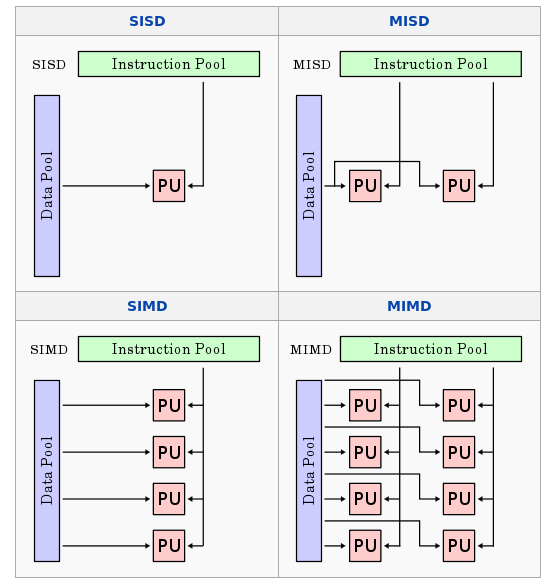
\includegraphics[width=0.80\textwidth]{figuras/flynn-ejemplo.png} \\
  \caption{Taxonom\'ia de Flynn: Comparaci\'on de las arquitecturas.} %
   \label{figFlynn1}
\end{figure}

\subsection{Modelos Paralelos}
Desde la perspectiva del sistema operativo, hay dos medios importantes de conseguir procesamiento paralelo: m\'ultiples procesos y m\'ultiples hilos. Un proceso es un programa en ejecuci\'on bajo control de un sistema operativo con un conjunto de recursos asociados. Estos recursos incluyen, pero no est\'an limitados a, estructuras de datos con informaci\'on del proceso, un espacio de direcciones virtuales conteniendo las instrucciones del programa y datos, y al menos un hilo de ejecuci\'on.  Un hilo es un camino de ejecuci\'on o flujo de control independiente dentro de un proceso, compuesto de un contexto (que incluye un conjunto de registros) y una secuencia de instrucciones a ejecutar\citep[Cap. 4]{Wad}. %OSO Hay una referencia de estas definiciones? %ANDRES est\'a sacado del libro que encontr\'e ``software optimization for high performance computing''.

En los sistemas de computaci\'on actuales existen distintos niveles de paralelismo. Por ejemplo, los procesadores VLIW y los RISC superescalares alcanzan paralelismo en el nivel de instrucci\'on (ejecutando varias instrucciones de bajo nivel al mismo tiempo)\citep{Grama, Wad}.\\
Para este trabajo de tesis utilizamos el t\'ermino ``procesamiento paralelo'' para indicar que hay m\'as de un hilo de ejecuci\'on ejecut\'andose en un \'unico programa. Esta definici\'on admite la implementaci\'on de procesamiento paralelo con m\'as de un proceso. Podemos as\'i considerar el procesamiento paralelo en tres categor\'ias\citep[Cap. 4]{Wad}:
\begin{itemize}
\item ``Paralelismo de procesos'': usar m\'as de un proceso para desempe\~nar un conjunto de tareas.
\item ``Paralelismo de hilos'': usar m\'ultiples hilos dentro de un \'unico proceso para ejecutar un conjunto de tareas.
\item ``Paralelismo h\'ibrido'': usar m\'ultiples procesos, donde al menos uno de ellos es un proceso paralelo con hilos, para desempe\~nar un conjunto de tareas.
\end{itemize}
Si bien se puede obtener paralelismo con m\'ultiples procesos, existen al menos dos razones potenciales para considerar paralelismo de hilos: conservaci\'on de recursos del sistema y ejecuci\'on m\'as r\'apida. Los hilos comparten acceso a los datos del proceso, archivos abiertos y otros atributos del proceso. Compartir datos e instrucciones puede reducir los requerimientos de recursos para un trabajo en particular. Por el contrario, una colecci\'on de procesos a menudo deber\'a duplicar las \'areas de datos e instrucciones en memoria para un trabajo.

\subsubsection{Conceptos b\'asicos de hilos}
La administraci\'on de hilos es m\'as simple que la de los procesos, ya que los hilos no poseen todos los atributos de un proceso. Pueden ser creados y destruidos mucho m\'as r\'apidamente que un proceso. Los hilos tienen otros atributos importantes, relacionados con el desempe\~no\citep[Cap. 4]{Wad}.\\

Un hilo ocioso es aquel que no tiene procesamiento para hacer y est\'a esperando su pr\'oximo conjunto de tareas. Por lo general el hilo es puesto en estado de espera (wait) de acuerdo con una variable de control, que puede tener dos valores, bloqueado o desbloqueado (debe esperar o puede continuar procesando, respectivamente).\\

Los hilos ociosos pueden ser suspendidos o quedar en espera activa (``spinning'' o ``busy waiting'')\citep[Cap. 4]{Wad}. Los hilos suspendidos liberan el procesador donde se estaban ejecutando. Los que est\'an en espera activa comprobar\'an repetidamente la variable para ver si ya est\'an desbloqueados, sin liberar el procesador para otros procesos. Como resultado de esto el rendimiento del sistema puede degradarse dr\'asticamente. Sin embargo, reiniciar un hilo suspendido puede llevar cientos, si no miles, de ciclos de procesador.\\

Otro atributo de los hilos es la afinidad, que consiste en la posibilidad de ligar un hilo con un mismo procesador al ser reiniciado luego de una suspensi\'on\citep[Cap. 4]{Wad}. La capacidad de manejar la afinidad permite mantener al hilo, siempre que sea posible, ejecutando sobre el mismo dispositivo de c\'omputo cada vez que vuelve al modo activo. De esta manera el hilo aprovecha los datos que hab\'ian sido puestos en cache durante su ejecuci\'on previa. De otro modo, deber\'ia volver a cargar todos los datos necesarios para reanudar su ejecuci\'on desde la memoria a la cache del nuevo procesador, con el costo de sobrecarga correspondiente.

\subsubsection{Hilos POSIX}
Reci\'en en 1995 se estableci\'o un est\'andar para la programaci\'on de hilos, a pesar de que los sistemas operativos ven\'ian implementando hilos desde hac\'ia d\'ecadas. El est\'andar es parte de la normativa ``POSIX (Portable Operating System Interface)'', en particular la porci\'on POSIX 1003.1c [REF] incluye las funciones y las Interfaces de Programaci\'on de Aplicaci\'on (``APIs'') que soportan m\'ultiples flujos de control dentro de un proceso. Los hilos creados y manipulados v\'ia este est\'andar son generalmente indicados como ``pthreads''. Con anterioridad al establecimiento de este est\'andar, las APIs de hilos eran espec\'ificas del fabricante del hardware, lo que hac\'ia muy dificil la portabilidad de las aplicaciones paralelas con hilos. Combinado con la complejidad de reescribir aplicaciones para utilizar y aprovechar el control expl\'icito de hilos, el resultado era que muy pocas aplicaciones paralelas utilizaban el modelo de hilos\citep[Cap. 4]{Wad}.
 
\subsubsection{Paralelismo basado en directivas del compilador}
El uso de directivas del compilador para conseguir paralelismo tiene el fin de aliviar la complejidad y los problemas de la portabilidad. En el paralelismo orientado a directivas, la mayor\'ia de los mecanismos paralelos se ponen en marcha a trav\'es del compilador (generaci\'on de hilos, generaci\'on de construcciones de sincronizaci\'on, etc.). Es decir, el compilador traduce las directivas de compilador en las llamadas al sistema necesarias para la administraci\'on de los hilos, y realiza cualquier reestructuraci\'on del c\'odigo que sea necesaria. Estas directivas proveen una manera simple de lograr paralelismo.

El est\'andar ``OpenMP''\citep{openmp} para directivas de compilador paralelas ha promovido el uso de esta forma de programaci\'on paralela. Antes de la aparici\'on de este est\'andar, las directivas de compilador eran espec\'ificas del fabricante del hardware, lo que dificultaba la portabilidad. 
Tanto la implementaci\'on expl\'icita de hilos paralelos (como pthreads) como el paralelismo basado en directivas (como OpenMP) se benefician del uso de memoria compartida.

\subsubsection{Paralelismo de memoria compartida}
El paralelismo de hilos depende de la existencia de la memoria compartida para la comunicaci\'on entre hilos. Otro modelo paralelo anterior tambi\'en utiliza memoria compartida, pero entre procesos. Este paralelismo de procesos t\'ipicamente se logra a trav\'es del uso de las llamadas al sistema ``fork()'' y ``exec()''  o sus an\'alogas. Por ello se lo denomina generalmente como el modelo ``fork/exec''. La memoria es compartida entre los procesos en virtud de las llamadas al sistema ``mmap()'' (derivada de Berkeley UNIX) o ``shmget()'' (de System V UNIX)\citep{Wad}.

\subsubsection{Pasaje de Mensajes}
El modelo fork/exec no implica la existencia de memoria compartida. Los procesos pueden comunicarse a trav\'es de interfaces de E/S tales como las llamadas al sistema ``read()'' y ``write()''. Esto puede darse a trav\'es de archivos regulares o a trav\'es de alguna otra forma est\'andar de comunicaci\'on entre procesos como los ``sockets''.  La comunicaci\'on a trav\'es de archivos resulta f\'acil entre procesos que comparten un sistema de archivos, pudiendo extenderse a varios sistemas al utilizar un sistema de archivos compartido como NFS. Los sockets son usualmente un medio de comunicaci\'on m\'as eficiente entre procesos ya que eliminan gran parte del costo de realizar operaciones sobre un sistema de archivos.

Estas dos t\'ecnicas comunes dependen de que el proceso escriba, o env\'ie, el dato a ser comunicado hacia un archivo o socket. Este acto de comunicaci\'on se considera un mensaje, esto es, el proceso emisor est\'a enviando un mensaje al proceso receptor. De ah\'i el nombre de pasaje de mensajes para este modelo.

Han existido diferentes implementaciones de bibliotecas de pasaje de mensajes, como PAR-MACS (para macros paralelas) y PVM (Parallel Virtual Machine)\citep{Wad,Grama}. Luego, en 1994, surge ``MPI''\citep{mpi} en un intento de brindar una API est\'andar de pasaje de mensajes. MPI pronto desplaz\'o a PVM y fue adoptando algunas de las ventajas de \'esta. A\'un cuando fue pensada principalmente para m\'aquinas de memoria distribuida, tiene la ventaja de que puede ser aplicada tambi\'en en m\'aquinas de memoria compartida. MPI est\'a destinado a paralelismo de procesos, no paralelismo de hilos.

\subsection{Infraestructuras de hardware para paralelismo}
Hist\'oricamente, las arquitecturas de computadoras paralelas han sido muy diversas. Existen a\'un diversas arquitecturas b\'asicas disponibles comercialmente hoy en d\'ia. En las siguientes secciones se dar\'a un panorama general de las arquitecturas paralelas.

\subsubsection{Clusters}
Un cluster es una colecci\'on interconectada de equipos independientes que son utilizadas como un solo recurso de computaci\'on. Un ejemplo com\'un de cluster es simplemente un conjunto de estaciones de trabajo conectadas por una red de \'area local\citep{Wad}.

Un aspecto positivo de un cluster es que en general cada nodo est\'a de por s\'i bien balanceado en t\'erminos de procesador, sistema de memoria y capacidades de E/S (ya que cada nodo es una computadora). Otra ventaja es el costo: un cluster puede consistir de estaciones de trabajo est\'andar, de f\'acil adquisici\'on. Del mismo modo, la interconexi\'on de los nodos puede ser resuelta con tecnolog\'ias de red local est\'andar como Ethernet, FDDI, etc. Los clusters tambi\'en resultan escalables, agreg\'andose nodos al sistema paralelo simplemente agregando m\'as estaciones de trabajo.\\

La capacidad y el desempe\~no de las interconexiones son dos puntos cr\'iticos de los clusters. Las operaciones que acceden a datos residentes en el mismo nodo donde est\'a ejecut\'andose la aplicaci\'on ser\'an relativamente r\'apidas; acceder a datos residentes en otros nodos resulta algo muy diferente. Los datos remotos deber\'an ser transferidos v\'ia llamadas al sistema para pasaje de mensajes. Esto implica los costos de la sobrecarga del mecanismo de llamadas al sistema y de la latencia de las comunicaciones, que dependen de la tecnolog\'ia de la red subyacente.\\

La administraci\'on del sistema presenta otro problema. Sin software especial para esta tarea, es complejo administrar el sistema. El software debe instalarse en cada nodo individual, lo cual puede ser un proceso lento y costoso (por ejemplo, si se necesita una licencia por cada nodo).\\

Otro aspecto es la carencia de una imagen \'unica del sistema. Nos referimos a la capacidad de que el cluster deba verse como un sistema solo y no como un conjunto de computadoras. Un usuario que ingresa en el sistema puede hacerlo siempre desde la misma estaci\'on de trabajo, con lo cual no ver\'a diferencias, pero si lo realiza desde distintas estaciones puede ver un ambiente muy distinto al cambiar de equipo. Por lo general se busca mantener los archivos utilizados por el usuario disponibles cada vez que ingrese, sin importar el equipo en el que est\'e, lo que trae mayor complejidad al cluster\citep{Wad}.

\subsubsection{Multiprocesadores Sim\'etricos (SMPs)}
Las computadoras multiprocesador suponen una alternativa para evitar los problemas de los clusters. En un multiprocesador, todos los procesadores acceden a todos los recursos de la m\'aquina. Cuando los procesadores son todos iguales y cada uno tiene acceso igualitario a los recursos de la computadora, el sistema se llama Multiprocesador Sim\'etrico (SMP por la sigla en ingl\'es)\citep{Wad}.

En los sistemas con modo dual de operaci\'on, las instrucciones privilegiadas se ejecutan en modo privilegiado o kernel. El proceso, que corre en modo de usuario, logra esto mediante llamadas al sistema, lo que provoca que el sistema operativo tome control sobre el hilo de ejecuci\'on del programa por un per\'iodo de tiempo. En un sistema multiprocesador, si s\'olo una CPU a la vez puede ejecutar en modo kernel, aparece un cuello de botella que transformar\'a la computadora multiprocesador en un sistema de un solo procesador.  Un equipo SMP debe ser capaz de que todos sus procesadores ejecuten en modo kernel. 

Al proveer un solo espacio de direcciones para las aplicaciones, un sistema SMP puede hacer el desarrollo de aplicaciones m\'as f\'acil que en un sistema con m\'ultiples e independientes espacios de direcciones como un cluster.

Un sistema SMP tendr\'a m\'ultiples procesadores, pero en realidad no tiene m\'ultiples sistemas de E/S o de memoria. Ya que en los SMP se tiene acceso igual o uniforme a la memoria, se dice que son m\'aquinas de Acceso Uniforme a Memoria (UMA - Uniform Memory Access). UMA implica que todos los procesadores pueden acceder a la memoria con la misma latencia. %OSO Aclarar que los modernos multicore son NUMA debido a la cache distribuida

\subsubsection{Buses y Crossbars}
Hay diferentes tecnolog\'ias que permiten conectar los dispositivos de c\'omputo entre s\'i y con el resto de los dispositivos del sistema. Un bus puede ser visto como un conjunto de l\'ineas de conexi\'on utilizado para conectar varios perif\'ericos de la computadora. La comunicaci\'on entre los recursos f\'isicos se hace com\'unmente con un bus. Generalmente hay dos grupos de buses en un sistema: buses de E/S y de memoria. Los de E/S t\'ipicamente son largos, pueden tener diferentes tipos de dispositivos conectados y normalmente acatan un est\'andar. Por el otro lado, los buses de memoria son cortos, de alta velocidad y usualmente optimizados, para maximizar el desempe\~no conjunto entre el procesador y la memoria. 

Otro m\'etodo com\'un de interconectar dispositivos es a trav\'es de crossbars. Un crossbar se asemeja a un conjunto m\'ultiples buses independientes que conectan cada uno de los m\'odulos en el multiprocesador. La implementaci\'on de un crossbar en hardware es sumamente complicada, debido a que debe permitir tantas comunicaciones independientes como sea posible mientras arbitra los pedidos m\'ultiples de acceso a un mismo recurso, tal como un banco de memoria. Todos los posibles caminos no conflictivos deben ser permitidos simult\'aneamente, pero esto supone un desarrollo complejo del hardware\citep{Wad}.

\section{C\'omputo de Altas Prestaciones}\label{sec:n2}
Luego de revisar el concepto de la computaci\'on paralela, las formas en que se categoriza y sus distintos modelos, definimos lo que podr\'ia llamarse una consecuencia de su evoluci\'on: el c\'omputo de altas prestaciones.

Un gran problema transversal a las Ciencias e Ingenier\'ias Computacionales es la aplicaci\'on eficiente de modernas herramientas de c\'omputo paralelo y distribuido. La respuesta a este problema est\'a condensada en el concepto de Computaci\'on de Altas Prestaciones (High Performance Computing, o HPC) que abarca todos aquellos principios, m\'etodos y t\'ecnicas que permiten abordar problemas con estructuras de c\'omputo complejas y de altos requerimientos.

El objetivo del proyecto HPC en la FaI es adquirir conocimientos para el dise\~no, desarrollo, gesti\'on y mejora de las tecnolog\'ias de hardware y software involucradas en la Computaci\'on de Altas Prestaciones (CAP) y sus aplicaciones en Ciencias e Ingenier\'ia Computacional.

Tradicionalmente, el \'ambito donde surg\'ian los productos de la ciencia y de la ingenier\'ia eran los laboratorios. Combinando la teor\'ia y la experimentaci\'on, con c\'alculos hechos a mano o apoy\'andose en herramientas de c\'alculo rudimentarias, se aplicaba el conocimiento de la f\'isica, la matem\'atica, la biolog\'ia, para obtener y validar nuevos conocimientos. La aparici\'on de las computadoras ofreci\'o una nueva y potente forma de hacer ciencia e ingenier\'ia: la ejecuci\'on de programas que utilizan modelos matem\'aticos y soluciones num\'ericas para resolver los problemas.

As\'i surgen herramientas como la simulaci\'on num\'erica, proceso de modelar matem\'aticamente un fen\'omeno de la realidad, y ejecutar experimentos virtuales a partir del modelo implementado en computador. En cada disciplina podemos encontrar experimentos que, por ser de alto costo, complejos, peligrosos o simplemente impracticables, hacen de la simulaci\'on num\'erica una herramienta de enorme valor. De la misma manera, las computadoras permiten la obtenci\'on de resultados concretos para problemas de c\'alculo imposibles de abordar en forma manual.

Hubo un tiempo cuando un analista num\'erico pod\'ia escribir c\'odigo para implementar un algoritmo. El c\'odigo era miope ya que era escrito solamente con la idea de implementar el algoritmo. Exist\'ia cierta consideraci\'on en la performance, pero generalmente era m\'as una idea de ahorrar la memoria de la computadora. La memoria era el comodity m\'as preciado en los albores de la computaci\'on. ``Tunear'' el c\'odigo para la arquitectura subyacente no era una consideraci\'on de primer orden.
A medida que las arquitecturas de computadoras evolucionaron, la tarea de codificaci\'on tuvo que ser ampliada para abarcar la explotaci\'on de la arquitectura. Esto fue necesario con el fin de obtener el rendimiento que se exige de c\'odigos de aplicaci\'on.

Los centros de computadoras de cada d\'ia mejoran los sistemas con m\'as procesadores y m\'as r\'apidos, m\'as memoria, y subsistemas de E/S mejorados, solo para descubrir que el rendimiento de la aplicaci\'on mejora un poco, si es que lo hace. Luego de algo de an\'alisis por los vendedores de sistemas o software, encontraron que sus aplicaciones simplemente no estaban dise\~nadas para explotar las mejoras en la arquitectura de la computadora. A pesar de los desarrolladores haber le\'ido textos sobre computaci\'on de alto desempe\~no y haber aprendido el significado de las palabras de moda, acr\'onimos, benchmarks y conceptos abstractos, nunca se les dieron los detalles sobre como dise\~nar o modificar realmente software que pueda beneficiarse de las mejoras en la arquitectura de la computadora.

\subsection{Ciencia e Ingenier\'ia Computacional}
La situaci\'on descripta en  los p\'arrafos anteriores ha dado auge a un nuevo campo interdisciplinario denominado Ciencia e Ingenier\'ia Computacional (Computational Science \& Engineering, CSE), que es la intersecci\'on de tres dominios: matem\'atica, ciencias de la computaci\'on, y las diferentes ramas de las ciencias o ingenier\'ias. La Ciencia e Ingenier\'ia Computacional usa herramientas de las ciencias de la computaci\'on y las matem\'aticas para estudiar problemas de las ciencias f\'isicas, sociales, de la Tierra, de la vida, de las diferentes disciplinas ingenieriles, etc.

Durante la presente d\'ecada, la Ciencia e Ingenier\'ia Computacional ha visto un desarrollo espectacular. Puede decirse que las tecnolog\'ias de c\'omputo y de comunicaciones han modificado el campo cient\'ifico de una manera que no admite el retroceso, sino que, al contrario, la superaci\'on y extensi\'on de esas tecnolog\'ias resulta vital para poder seguir haciendo ciencias como las conocemos hoy.

Gracias a estos avances tecnol\'ogicos los cient\'ificos pueden trascender sus anteriores alcances, extender sus resultados y abordar nuevos problemas, antes intratables. Entre los m\'etodos de la Ciencia e Ingenier\'ia Computacional se incluyen:

\begin{itemize}
\item Simulaciones num\'ericas, con diferentes objetivos:
     \begin{itemize}
      \item Reconstrucci\'on y comprensi\'on los eventos naturales conocidos: terremotos, incendios forestales, maremotos, etc.
      \item Predicci\'on del futuro o de situaciones inobservables: predicci\'on del tiempo, comportamiento de part\'iculas subat\'omicas.
     \end{itemize}
\end{itemize} 
\begin{itemize}
\item Ajustes de modelos y an\'alisis de datos
      \begin{itemize}
      \item Sintonizaci\'on de modelos o resoluci\'on de ecuaciones para reflejar observaciones, sujetas a las limitaciones del modelo: prospecci\'on geof\'isica, lingü\'istica computacional.
      \item Modelado de redes, en particular aquellas que conectan individuos, organizaciones, o sitios web.
      \item Procesamiento de im\'agenes, inferencia de conceptos y discriminantes: detecci\'on de caracter\'isticas del terreno, de procesos climatol\'ogicos, reconocimiento de patrones gr\'aficos
      \end{itemize}
\end{itemize}
\begin{itemize}
\item Optimizaci\'on
      \begin{itemize}
      \item An\'alisis y mejoramiento de escenarios conocidos, como procesos t\'ecnicos y de manufactura.
      \end{itemize}
\end{itemize}
A estos m\'etodos, cuya aplicaci\'on hoy ya es corriente en las ciencias e ingenier\'ias, se suman ciertos problemas, denominados ``grandes desaf\'ios'', y cuya soluci\'on tiene amplio impacto sobre el desarrollo de esas disciplinas. Estos problemas pueden ser tratados por la aplicaci\'on de t\'ecnicas y recursos de Computaci\'on de Altas Prestaciones. Algunos de los campos donde aparecen estos problemas son:

\begin{itemize}
\item Din\'amica de fluidos computacional, para el dise\~no de aeronaves, la predicci\'on del tiempo a t\'erminos cortos o largos, para la recuperaci\'on eficiente de minerales, y muchas otras aplicaciones.
\item C\'alculos de estructuras electr\'onicas, para el dise\~no de nuevos materiales como catal\'iticos qu\'imicos, agentes inmunol\'ogicos, o superconductores.
\item C\'omputos que permitan comprender la naturaleza fundamental de la materia y de los procesos de la vida.
\item Procesamiento simb\'olico, incluyendo reconocimiento del habla, visi\'on por computadora, comprensi\'on del lenguaje natural, razonamiento automatizado y herramientas varias para dise\~no, manufactura y simulaci\'on de sistemas complejos.
\end{itemize}
La resoluci\'on de estos problemas involucra conjuntos masivos de datos, una gran cantidad de variables y complejos procesos de c\'alculo; por otro lado, es de car\'acter abierto, en el sentido de que siempre aparecer\'an escenarios de mayor porte o mayor complejidad para cada problema. Estos m\'etodos y sus t\'ecnicas particulares exigen la utilizaci\'on de recursos de computaci\'on hasta hoy excepcionales, como lo han sido las supercomputadoras, los multiprocesadores y la colaboraci\'on de una gran cantidad de computadoras a trav\'es de las redes, en diferentes niveles de agregaci\'on como clusters, multiclusters y grids.

\section{Fortran}\label{sec:n3}
Muy popular en la programaci\'on cient\'ifica y la computaci\'on de alto desempe\~no (HPC), el lenguaje Fortran surge a mediados de la d\'ecada de 1950, siendo uno de los lenguajes de programaci\'on m\'as antiguos utilizados a\'un hoy por cient\'ificos de todo el mundo. Se lo clasifica como un lenguaje de programaci\'on de alto nivel (considerado el primero de ellos en aparecer), de prop\'osito general e imperativo. La programaci\'on imperativa describe un programa en t\'erminos del estado del programa y las sentencias que cambian dicho estado, como descripto por una m\'aquina de Turing.  

Fue desarrollado para aplicaciones cient\'ificas y de ingenier\'ia, campos que domin\'o r\'apidamente, siendo durante todo este tiempo ampliamente utilizado en \'areas de c\'omputo intensivo, tales como el an\'alisis de elementos finitos, predicci\'on num\'erica del clima, din\'amica de fluidos computacional o f\'isica computacional. 
Ampliamente adoptado por cient\'ificos para escribir programas num\'ericamente intensivos, impuls\'o a los constructores de compiladores a generar c\'odigo m\'as r\'apido y eficiente. La inclusi\'on de un tipo de dato complejo (COMPLEX) lo hizo especialmente apto para aplicaciones t\'ecnicas como la Ingenier\'ia El\'ectrica. 

En las \'areas cient\'ificas, con t\'ipicos problemas de c\'alculo intensivo, una vez que un programa alcanza un estado de computaci\'on correcta (i.e. arroja los resultados deseados), no suelen ocurrir modificaciones del c\'odigo. En el caso de Fortran, su adopci\'on por la comunidad cient\'ifica deriv\'o en la construcci\'on de programas que permanecen vigentes tras 20, 30 y hasta 40 a\~nos. Estos constituyen lo que denominamos ``Legacy Software''. Se ha definido al Legacy Software como:

\begin{itemize}
\item ``Software cr\'itico que no puede ser modificado eficientemente''\citep{Gold}.
\item ``Cualquier sistema de informaci\'on que significativamente resiste las modificaciones y la evoluci\'on para alcanzar requerimientos de negocio nuevos y constantemente cambiantes''\citep{Brod}. 
\end{itemize}
Algunas caracter\'isticas de los sistemas legacy son:

\begin{itemize}
\item La resistencia al cambio del software.
\item La complejidad inherente.
\item La tarea crucial desempe\~nada por el software en la organizaci\'on.
\item El tama\~no del sistema, generalmente mediano o grande.
\end{itemize}
Es com\'un hallar software hecho en Fortran que ha estado ejecut\'andose en ambientes de producci\'on por d\'ecadas. Durante ese per\'iodo, el software se deteriora gradualmente y puede necesitar cambios de diferente tipo, como: mejoras, correcciones, adaptaciones y prevenciones. Para todas estas tareas se necesita conocimiento y comprensi\'on del sistema. En la era multi-core y many-core, los cambios de software se hacen m\'as y m\'as complejos\citep{MMen}.
%OSO Est\'a bien esta frase?. la siguiente- cita a donde es nombrada
Debido a que Fortran ha estado tantos a\~nos vigente, ha pasado por un proceso particular de estandarizaci\'on en el cual cada versi\'on previa del est\'andar cumple con el vigente. Este proceso de estandarizaci\'on permite que un programa en Fortran 77 compile en los compiladores modernos de Fortran 2008\citep{MMen}. Gracias a estas caracter\'isticas es que el lenguaje est\'a, a\'un hoy y a pesar de ser relativamente poco visible, en una posici\'on s\'olida y bien definida. Actualmente hay un gran conjunto de programas Fortran ejecut\'andose en ambientes productivos de universidades, empresas e instituciones de gobierno. Algunos buenos ejemplos son programas de modelo clim\'atico, simulaciones de terremotos, simulaciones magnetohidrodin\'amicas, etc. La mayor\'ia de estos programas han sido construidos a\~nos o d\'ecadas atr\'as y sus usuarios necesitan que sean modernizados, mejorados y/o actualizados. Esto tambi\'en implica que estos programas sean capaces de aprovechar las arquitecturas de procesadores modernas y, espec\'ificamente, el equipamiento para procesamiento num\'erico.

\subsection{Evoluci\'on del lenguaje}
Fortran ha evolucionado de una release inicial con 32 sentencias para la IBM 704, entre los que estaban el condicional IF y el IF aritm\'etico de 3 v\'ias, el salto GO TO, el bucle DO, comandos para E/S tanto formateada como sin formato (FORMAT, READ, WRITE, PRINT, READ TAPE, READ DRUM, etc), y de control del programa (PAUSE, STOP, CONTINUE), y tipos de datos todos num\'ericos, hasta llegar al \'ultimo estandar Fortran, ISO/IEC 1539-1:2010, conocido informalmente como Fortran 2008, donde fueron incorpor\'andose caracter\'isticas como tipos de datos CHARACTER, definici\'on de arrays, subrutinas, funciones, recursividad, modularidad, hasta nuevas sentencias que soportan la ejecuci\'on de alta performance como DO CONCURRENT, coarrays (un modelo de ejecuci\'on paralela). Si se desea ahondar en la definici\'on del est\'andar Fortran el mismo puede encontrarse en el sitio de NAG (The Numerical Algorithms Group) quienes alojan el home oficial para los est\'andares de Fortran\footnote{\url{http://www.nag.co.uk/sc22wg5/}}.

El lenguaje utilizado en el programa de estudio de este trabajo de tesis est\'a basado en el est\'andar Fortran 77. Se presentan en el anexo A las sentencias de Fortran m\'as utilizadas en la aplicaci\'on objeto de estudio.

\section{OpenMP}\label{sec:n4}
OpenMP es una Interfaz de Programaci\'on de Aplicaciones, o API por sus siglas en Ingles, la cual provee un modelo portable y escalable para el desarrollo de aplicaciones paralelas de memoria compartida. La API soporta C/C++ y Fortran en una gran variedad de arquitecturas. Es utilizada para de manera directa aplicar multihilos en memoria compartida\footnote{\url{https://computing.llnl.gov/tutorials/openMP/}}.

La especificaci\'on de OpenMP\citep{openmp} pertenece, es escrita y mantenida por la OpenMP Architecture Review Board, que es la uni\'on de las compa\~n\'ias que tienen participaci\'on activa en el desarrollo del est\'andar para la interfaz de programaci\'on en memoria compartida\citep{Her}.

No es un nuevo lenguaje de programaci\'on, sino que es una notaci\'on que puede ser agregada a un programa secuencial en Fortran, C o C++ para describir como el trabajo debe ser compartido entre los hilos que se ejecutaran en diferentes procesadores o n\'ucleos y para organizar el acceso a los datos compartidos cuando sea necesario.
La inserci\'on apropiada de las caracter\'isticas de OpenMP en un programa secuencial permitir\'a a muchas, si no a la mayor\'ia, de las aplicaciones beneficiarse de una arquitectura de memoria compartida, a menudo con m\'inimas modificaciones al c\'odigo.
Uno de los factores del \'exito de OpenMP es que es comparativamente sencillo de usar, ya que el trabajo m\'as complicado de armar los detalles del programa paralelo son dejados para el compilador. Tiene adem\'as la gran ventaja de ser ampliamente adoptado, de manera que una aplicaci\'on OpenMP va a poder ejecutarse en muchas plataformas diferentes\citep[Cap. 1]{Chap}.

Las directivas de OpenMP permiten al usuario indicarle al compilador que instrucciones ejecutar en paralelo y como distribuir las mismas entre los hilos que van a ejecutar el c\'odigo.
Una de estas directivas es una instrucci\'on en un formato especial que es entendido por compiladores OpenMP solamente. De hecho luce como un comentario para un compilador Fortran regular, o una diretiva pragma para un compilador C/C++, de manera que el programa puede ejecutarse como lo hac\'ia previamente si el compilador no conoce OpenMP.
Generalmente se puede r\'apida y f\'acilmente crear programas paralelos confiando en la implementaci\'on para que trabaje los detalles de la ejecuci\'on paralela. Pero no siempre es posible obtener alta performance con una inserci\'on sencilla, incremental de directivas OpenMP en un c\'odigo secuencial. Por esta raz\'on OpenMP incluye varias caracter\'isticas que habilitan al programador a especificar m\'as detalle en el c\'odigo paralelo.

\subsection{La idea de OpenMP}
Un hilo es una entidad en tiempo de ejecuci\'on que es capaz de ejecutar independientemente un flujo de instrucciones. OpenMP trabaja en un cuerpo m\'as grande de trabajo que soporta la especificaci\'on de programas para ser ejecutados por una colecci\'on de hilos cooperativos. El sistema operativo crea un proceso para ejecutar un programa: reservar\'a algunos recursos para este proceso, incluyendo p\'aginas de memoria y registros para almacenar valores de objetos. Si multiples hilos colaboran para ejecutar un programan, compartir\'an los recursos, incluyendo el espacio de direcciones, del correspondiente proceso. Los hilos individuales necesitan muy pocos recursos por si mismos: un contador de programa y un \'area de memoria para guardar variables especificas del hilo (incluyendo registros y una pila)\citep[Cap. 2]{Chap}.
OpenMP intenta proveer facilidad de programaci\'on y ayudar al usuario a evitar un n\'umero de potenciales errores de programaci\'on, ofreciendo un enfoque estructurado para la programaci\'on multihilo. Soporta el modelo de programaci\'on llamado fork-join, el cual podemos ver en la Fig. \ref{figFork1}.

\begin{figure}[h!]%[htp]
  \centering
  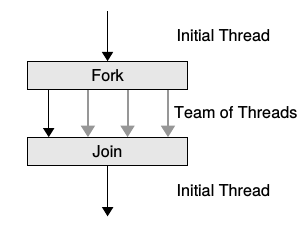
\includegraphics[width=0.50\textwidth]{figuras/fork-join1.png} \\
  \caption{Modelo fork-join} %
   \label{figFork1}
\end{figure}

Bajo este enfoque, el programa inicia como un solo hilo de ejecuci\'on (denominado hilo inicial), igual que un programa secuencial. Siempre que se encuentre una construcci\'on paralela de OpenMP por el hilo mientras ejecuta su programa, se crea un equipo de hilos (esta es la parte fork), se convierte en el maestro del equipo, y colabora con los otros miembros del equipo para ejecutar el c\'odigo din\'amicamente encerrado por la construcci\'on. Al final de la construcci\'on, solo el hilo original, o maestro del equipo, continua; todos los dem\'as terminan (esta es la parte join). Cada porci\'on del c\'odigo encerrada por una construcci\'on paralela es llamada una regi\'on paralela.

\subsection{Conjunto de construcciones paralelas}
La API OpenMP comprende un conjunto de directivas del compilador, rutinas de bibliotecas de tiempo de ejecuci\'on, y variables de ambiente para especificar paralelismo de memoria compartida. Muchas de las directivas son aplicadas a un bloque estructurado de c\'odigo, una secuencia de sentencias ejecutables con una sola entrada en la parte superior y una sola salida en la parte inferior en los programas Fortran, y una sentencia ejecutable en C/C++ (que puede ser una composici\'on de sentencias con una sola entrada y una sola salida). En otras palabras, el programa no puede ramificarse dentro o fuera de los bloques de c\'odigo asociados con directivas. En Fortran el inicio y el final del bloque aplicable de c\'odigo son marcados expl\'icitamente por una directiva OpenMP\citep[Cap. 2]{Chap}.

\subsubsection{Crear equipos de Hilos}
Un equipo de hilos es creado para ejecutar el c\'odigo en una regi\'on paralela de un programa OpenMP. El programador simplemente especifica la regi\'on paralela insertando una directiva \emph{parallel} inmediatamente antes del c\'odigo que debe ser ejecutado en paralelo para marcar su inicio; en los programas Fortran el final tambi\'en es indicado por una directiva end parallel. Informaci\'on adicional puede ser provista junto con la diretiva \emph{parallel}, como habilitar a los hilos a tener copias privadas de alg\'un dato por la duraci\'on de la regi\'on paralela. El final de una regi\'on paralela es una barrera de sincronizaci\'on impl\'icita: esto significa que ning\'un hilo puede progresar hasta que todos los dem\'as hilos del equipo hayan alcanzado este punto del programa\citep[Cap. 2]{Chap}. Es posible realizar anidado de regiones paralelas.

\subsubsection{Compartir trabajo entre Hilos}
Si el programador no especifica como se compartir\'a el trabajo en una regi\'on paralela, todos los hilos ejecutar\'an el c\'odigo completo redundantemente, sin mejorar los tiempos del programa. Para ello OpenMP cuenta con directivas para compartir trabajo que permiten indicar como se distribuir\'a el computo en un bloque de c\'odigo estructurado entre los hilos. A menos que el programador lo indique expl\'icitamente, una barrera de sincronizaci\'on existe impl\'icitamente al final de las construcciones de trabajo compartido\citep[Cap. 2]{Chap}.

Probablemente el m\'etodo m\'as com\'un de trabajo compartido es distribuir el trabajo en un bucle DO (Fortran) o for (C/C++) entre los distintos hilos de un equipo. El programador inserta la directiva apropiada inmediatamente antes de los bucles que vayan a ser compartidos entre los hilos dentro de una regi\'on paralela.
Todas las estrategias de OpenMP para compartir el trabajo en un bucle asignan uno o m\'as conjuntos disjuntos de iteraciones a cada hilo. El programador puede, si as\'i lo desea, especificar el m\'etodo para particionar el conjunto de iteraci\'on.

\subsubsection{Modelo de memoria de OpenMP}
OpenMP se basa en el modelo de memoria compartida, por ello, por defecto los datos son compartidos por todos los hilos y son visibles para todos. A veces es necesario tener variables que tienen valores espec\'ificos por hilo. Cuando cada hilo tiene una copia propia de una variable, donde potencialmente tenga valores distintos en cada uno de ellos, decimos que la variable es privada. Por ejemplo, cuando un equipo de hilos ejecuta un bucle paralelo  cada hilo necesita su propio valor de la variable de control de iteraci\'on. Este caso es tan importante que el propio compilador fuerza que as\'i sea; en otros casos el programador es quien debe determinar cuales variables son compartidas y cuales privadas\citep[Cap. 2]{Chap}.

\subsubsection{Sincronizaci\'on de Hilos}
Sincronizar los hilos es necesario en ocasiones para asegurar el acceso en orden a los datos compartidos y prevenir corrupci\'on de datos. Asegurar la coordinaci\'on de hilos necesaria es uno de los desaf\'ios m\'as fuertes de la programaci\'on de memoria compartida\citep[Cap. 2]{Chap}. OpenMP provee, por defecto, sincronizaci\'on impl\'icita haciendo que los hilos esperen al final de una construcci\'on de trabajo compartido o regi\'on paralela hasta que todos los hilos en el equipo terminan su porci\'on de trabajo. M\'as dif\'icil de conseguir en OpenMP es coordinar las acciones de un subconjunto de los hilos ya que no hay soporte expl\'icito para esto.
Otras veces es necesario asegurar que solo un hilo a la vez trabaja en un bloque de c\'odigo. OpenMP  tiene varios mecanismos que soportan este tipo de sincronizaci\'on.

\subsubsection{Otras caracteristicas}
Subrutinas y funciones pueden complicar la utilizaci\'on de APIs de Programaci\'on Paralela. Una de las caracter\'isticas innovativas de OpenMP es el hecho de que las directivas pueden ser insertadas dentro de procedimientos que son invocados desde dentro de una regi\'on paralela.\\
Para algunas aplicaciones puede ser necesario controlar el n\'umero de hilos que ejecutan la regi\'on paralela. OpenMP permite al programador especificar este n\'umero previo a la ejecuci\'on del programa a trav\'es de una variable de ambiente, luego de que el c\'omputo a iniciado a trav\'es de una librer\'ia de rutinas, o al comienzo de regiones paralelas. Si no se hace esto, la implementaci\'on de OpenMP utilizada elegir\'a el n\'umero de hilos a utilizar\citep[Cap. 2]{Chap}.

\section{OpenMP en Fortran}\label{sec:n5}
Fueron presentados Fotran y OpenMP, en esta secci\'on se ve como se complementan, mostrando cuales es el formato de las directivas de OpenMP en Fortran.

\subsection{Centinelas para directivas de OpenMP y compilaci\'on condicional}

El est\'andar OpenMP ofrece la posibilidad de usar el mismo c\'odigo fuente con un compilador que implementa OpenMP como con uno normal. Para ello debe ocultar las directivas y comandos de una manera que un compilador normal no pueda verlas. Para ello existen las siguientes directivas centinelas\citep{Her}
\begin{lstlisting}[style=For, numbers=none]
 !$OMP

 !$
\end{lstlisting}
Como el primer caracter es un signo de exclamaci\'on ``!'', un compilador normal va a interpretar las l\'ineas como comentarios y va a ignorar su contenido. Pero un compilador compatible con OpenMP identificar\'a la sentencia y proceder\'a como sigue\citep{Her}
\begin{itemize}
\item !\$OMP : el compilador compatible con OpenMP sabe que la informaci\'on que sigue en la l\'inea es una directiva OpenMP. Se puede extender una directiva en varias l\'ineas utilizando el mismo centinela frente a las siguientes l\'ineas y usando el m\'etodo est\'andar de Fortran para partir l\'ineas de c\'odigo:
   \begin{lstlisting}[style=For, numbers=none]
        !$OMP PARALLEL DEFAULT(NONE) SHARED(A, B) &
        !$OMP REDUCTION(+:A)
   \end{lstlisting}
\end{itemize}
Es obligatorio incluir un espacio en blanco entre la directiva centinela y la directiva OpenMP que le sigue, sino la l\'inea ser\'a interpretada como un comentario.
\begin{itemize}
\item !\$ : la l\'inea correspondiente se dice que est\'a afectada por una compilaci\'on condicional. Quiere decir que su contenido estar\'a disponible para el compilador en caso de que sea compatible con OpenMP. Si esto ocurre, los dos caracteres del centinela son reemplazados por dos espacios en blanco para que el compilador tenga en cuenta la l\'inea. Como en el caso anterior podemos extender la l\'inea en varias l\'ineas como sigue:
   \begin{lstlisting}[style=For, numbers=none]
	!$ interval = L * OMP_get_thread_num() / &
	!$                       (OMP_get_num_threads() - 1)
   \end{lstlisting}
\end{itemize}
Nuevamente el espacio en blanco es obligatorio entre la directiva de compilaci\'on condicional y el c\'odigo fuente que le sigue.

\subsection{El constructor de regi\'on paralela}
La directiva m\'as importante en OpenMP es la que define las llamadas regiones paralelas. Para entender mejor qu\'e es la regi\'on paralela se puede observar una representaci\'on en la Fig. \ref{figRegpar} tomada de \citep{Her}.\\
Podemos definir sencillamente que cuando se crea la regi\'on paralela se crean los hilos que ejecutaran paralelamente el c\'odigo que est\'e definido dentro de la misma.

\begin{figure}[h!]%[htp]
  \centering
  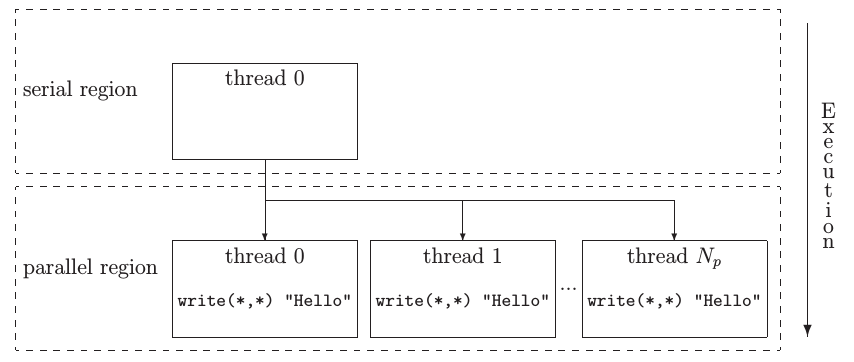
\includegraphics[width=0.80\textwidth]{figuras/reg-paralela1.png} \\
  \caption{Representaci\'on de la Regi\'on Paralela.} %
  \label{figRegpar}
\end{figure}

Ya que la regi\'on paralela necesita ser creada/abierta y destruida/cerrada, dos directivas son necesarias en Fotran: !\$OMP PARALLEL / !\$OMP END PARALLEL.
El c\'odigo de la Fig. \ref{figRegpar} se puede ver a continuaci\'on:

\begin{lstlisting}[style=For, numbers=none]
!$OMP PARALLEL 
	  write(*,*) ``Hola''
!$OMP END PARALLEL
\end{lstlisting}

Como el c\'odigo entre las dos directivas es ejecutado por cada hilo, el mensaje \emph{Hola} aparece en la pantalla tantas veces como hilos est\'en siendo usados en la regi\'on paralela.
Al comienzo de la regi\'on paralela es posible imponer cl\'ausulas que fijan ciertos aspectos de la manera en que la regi\'on paralela va a trabajar, por ejemplo el alcance de las variables, el n\'umero de hilos, etc. La sintaxis a usar es la siguiente:
\begin{lstlisting}[style=For, numbers=none]
	!$OMP PARALLEL  clause1 clause2 ...
	...
	!\$OMP END PARALLEL
\end{lstlisting}
Las cl\'ausulas permitidas en la directiva de apertura !\$OMP PARALLEL son las siguientes:
\begin{itemize}
\item PRIVATE(lista)
\item SHARED(lista)
\item DEFAULT( PRIVATE | SHARED | NONE )
\item FIRSTPRIVATE(lista)
\item COPYIN(lista)
\item REDUCTION(operador:lista)
\item IF(expresi\'on\_escalar\_l\'ogica)
\item NUM\_THREADS(expresi\'on\_escalar\_entera)
\end{itemize}
La directiva !\$OMP END PARALLEL indica el final de la regi\'on paralela, la barrera impl\'icita mencionada antes en el capitulo. En este punto es donde ocurre la sincronizaci\'on entre el equipo de hilos y son terminados todos excepto el hilo maestro que continua con la ejecuci\'on del programa.

\subsection{Directiva !\$OMP DO}
Es una directiva de trabajo compartido, por lo cual al encontrarla en el c\'odigo el trabajo es distribuido en un equipo de hilos. Debe ser ubicada dentro del alcance de una regi\'on paralela para ser efectiva, si no, la directiva a\'un funcionar\'a pero el equipo ser\'a de un solo hilo. Esto se debe a que la creaci\'on de nuevos hilos es una tarea reservada a la directiva de creaci\'on de la regi\'on paralela.
Esta directiva hace que el bucle \emph{Do} inmediato sea ejecutado en paralelo.
Por ejemplo:
\begin{lstlisting}[style=For, numbers=none]
	!$OMP DO
		do 1   i = 1, 1000
		...
	  1 continue
	!$OMP END DO
\end{lstlisting}
distribuye el bucle \emph{Do} entre los diferentes hilos, cada hilo computa una parte de las iteraciones.
Por ejemplo si usamos 10 hilos, entonces generalmente cada hilo computa 100 iteraciones del bucle do. El hilo 0 desde 1 a 100, el hilo 1 desde 101 a 200 y as\'i sucesivamente. Podemos ver esto en la Fig. \ref{figRegparDo} tomada de \citep{Her}.

\begin{figure}[h!]%[htp]
  \centering
  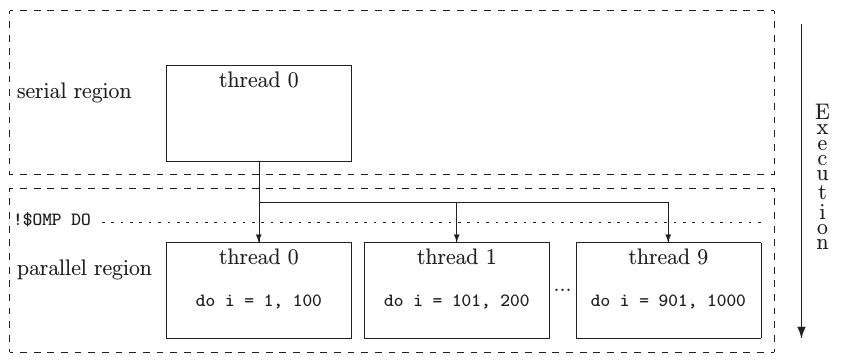
\includegraphics[width=0.80\textwidth]{figuras/reg-paralelaDo.png} \\
  \caption{Representaci\'on gr\'afica de la directiva \emph{OMP DO}.} %
  \label{figRegparDo}
\end{figure}

Dentro del trabajo de esta tesis es la directiva principal al tratarse los bucles \emph{Do} de una de las principales construcciones utilizadas en el programa estudiado.

La directiva !\$OMP DO tiene asociadas cl\'ausulas al igual que la directiva parallel, que permiten indicar el comportamiento de la construcci\'on de trabajo compartido. La sintaxis es similar:
\begin{lstlisting}[style=For, numbers=none]
	!$OMP DO clause1 clause2 ...
	...
	!$OMP END DO end_clause
\end{lstlisting}
Las cl\'ausulas de inicio pueden ser cualquiera de las siguientes:
\begin{itemize}
\item PRIVATE(lista)
\item FIRSTPRIVATE(lista)
\item LASTPRIVATE(lista)
\item REDUCTION(operador:lista)
\item SCHEDULE(tipo, pedazo)
\item ORDERED
\end{itemize}
Adicionalmente a estas cl\'ausulas de inicio, se puede agregar a la directiva de cierre la cl\'ausula NOWAIT para evitar la sincronizaci\'on impl\'icita. Tambi\'en se evita el refresco de las variables compartidas, impl\'icito en la directiva de cierre, por lo que se debe tener cuidado de cuando utilizar la cl\'ausula NOWAIT. Se pueden evitar problemas con la directiva de OpenMP !\$OMP FLUSH que fuerza el refresco de las variables compartidas en memoria por los hilos.

\subsection{Clausulas Atributo de Alcance de Datos}
\subsubsection{PRIVATE(lista)}
A veces, ciertas variables van a tener valores diferentes en cada hilo. Esto s\'olo es posible si cada hilo tiene su propia copia de la variable. Esta cl\'ausula fija que variables van a ser consideradas variables locales de cada hilo. Por ejemplo, para indicar que las variables a y b tendr\'an diferentes valores en cada hilo, i.e., ser\'an locales/privadas a cada hilo, utilizamos el siguiente c\'odigo: 

\begin{lstlisting}[style=For, numbers=none]
    !$OMP PARALLEL PRIVATE(a, b)
\end{lstlisting}

%\begin{figure}[h!]%[htp][style=For, numbers=none]
%  \centering
%    \begin{lstlisting}[style=For, numbers=none]
%        		!$OMP PARALLEL PRIVATE(a, b)
%    \end{lstlisting}
%  \caption{Ejemplo cl\'ausula PRIVATE.} %
%  \label{figPriv1}
%\end{figure}

Cuando una variable se declara como privada, un nuevo objeto del mismo tipo es declarado por cada hilo del equipo y usado por cada hilo dentro del alcance de la directiva que lo declare (la regi\'on paralela en el ejemplo anterior) en lugar de la variable original. El c\'odigo anterior se representa en la Fig. \ref{figRegparPriv} de \citep{Her}.

\begin{figure}[h!]%[htp]
  \centering
  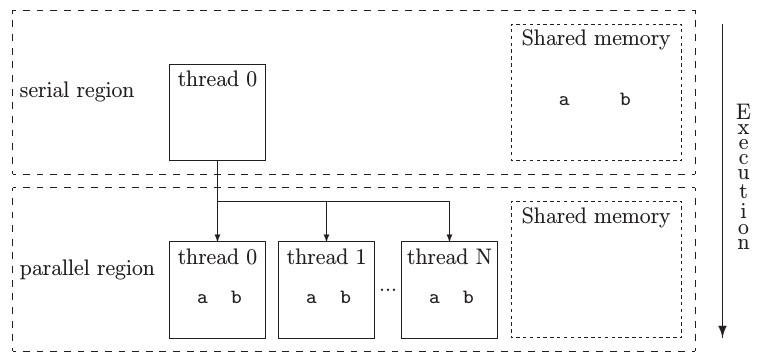
\includegraphics[width=0.80\textwidth]{figuras/reg-paralelaPriv.png} \\
  \caption{Representaci\'on gr\'afica de la cl\'ausula PRIVATE.} %
  \label{figRegparPriv}
\end{figure}

El hecho de que un nuevo objeto es creado por cada hilo puede ser algo que genere mucho consumo de recursos. Por ejemplo, si se utiliza un array de 5Gb (algo com\'un en simulaciones num\'ericas directas y otras) y es declarado como privado en una regi\'on paralela con un equipo de 10 hilos, entonces el requerimiento de memoria ser\'a de 55Gb, algo no disponible en todas las maquinas SMP.

Las variables utilizadas como contadores en los bucles \emph{Do} o comandos \emph{forall}, o son declaradas THREADPRIVATE, se convierten autom\'aticamente en privadas para cada hilo, a\'un cuando no hayan sido declaradas en un cl\'ausula PRIVATE.

\subsubsection{SHARED(lista)}

Contrario a lo visto en la situaci\'on previa, a veces hay variables que deben estar disponibles para todos los hilos dentro del alcance de una directiva, debido a que su valor es necesario para todos los hilos o porque todos los hilos deben actualizar su valor. Por ejemplo:
\begin{lstlisting}[style=For, numbers=none]
      !$OMP PARALLEL SHARED(c, d)
\end{lstlisting}
\noindent indica que las variables c y d son vistas por todos los hilos en el alcance de las directivas !\$OMP PARALLEL / !\$OMP END PARALLEL. Podemos observar en la Fig. \ref{figRegparShar} de \citep{Her} la representaci\'on deL ejemplo.

\begin{figure}[h!]%[htp]
  \centering
  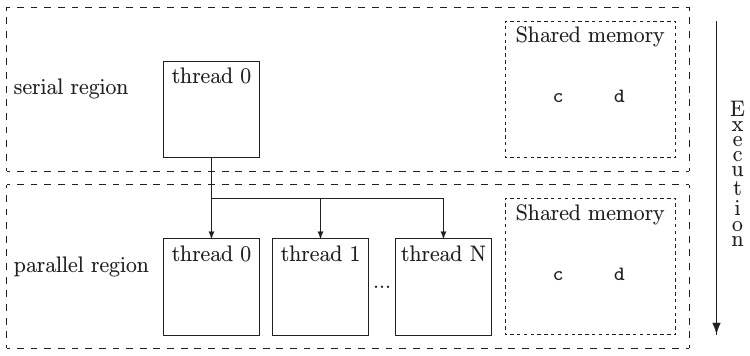
\includegraphics[width=0.80\textwidth]{figuras/reg-paralelaShar.png} \\
  \caption{Representaci\'on gr\'afica de la cl\'ausula SHARED.} %
  \label{figRegparShar}
\end{figure}

Una variable declarada como compartida (shared) no consume recursos extras, ya que no se reserva nueva memoria y su valor antes de la directiva inicial es conservado. Es decir que todos los hilos acceden a la misma ubicaci\'on de memoria para leer y escribir la variable.
Debido a que m\'as de un hilo puede escribir en la misma ubicaci\'on de memoria al mismo tiempo, resulta en un valor indefinido de la variable. A esto se lo llama una condici\'on de carrera, y debe ser siempre evitado por el programador. 

\subsubsection{DEFAULT ( PRIVATE \textbar SHARED \textbar NONE )}
Cuando la mayor\'ia de las variables dentro del alcance de una directiva va a ser privada o compartida, entonces ser\'ia engorroso incluir todas ellas en una de las cl\'ausulas previas. Para evitar esto, es posible especificar que har\'a OpenMP cuando no se especifica nada sobre una variable, es posible especificar un comportamiento por defecto. Por ejemplo:
\begin{lstlisting}[style=For, numbers=none]
      !\$OMP PARALLEL DEFAULT(PRIVATE) SHARED(a)
\end{lstlisting}
\noindent indica que todas las variables excepto ``a'' van a ser privadas, mientras que ``a'' ser\'a compartida por todos los hilos dentro del alcance de la regi\'on paralela. Si no se especifica ninguna cl\'ausula DEFAULT, el comportamiento por defecto es como si DEFAULT(SHARED) fuera especificado. Como veremos en el capitulo 3 de este trabajo de tesis, esto puede variar en implementaciones y debe ser investigado m\'as a fondo.
A las opciones PRIVATE y SHARED se le agrega una tercera: NONE. Especificando DEFAULT(NONE) requiere que cada variable en el alcance de la directiva debe ser expl\'icitamente listada en una de las cl\'ausulas PRIVATE o SHARED al principio del alcance de la directiva (exceptuando variables declaradas THREADPRIVATE o los contadores de los bucles).

\subsubsection{FIRSTPRIVATE(lista)}
Como mencionamos previamente, las variables privadas tienen un valor indefinido al comienzo del alcance de un par de directivas de inicio y cierre. Pero a veces es de inter\'es que esas variables locales tengan el valor de la variable original antes de la directiva de inicio. Esto se consigue incluyendo la variable en una cl\'ausula FIRSTPRIVATE como:
\begin{lstlisting}[style=For, numbers=none]
	a = 2
	b = 1
	!$OMP PARALLEL PRIVATE(a) FIRSTPRIVATE(b)
\end{lstlisting}
En este ejemplo, la variable ``a'' tiene un valor indefinido al inicio de la regi\'on paralela, mientras que ``b'' tiene el valor especificado en la regi\'on serial precedente, es decir ``b = 1''. Podemos ver este ejemplo en la Fig. \ref{figRegparVarPriv} tomada de \citep{Her}.

\begin{figure}[h!]%[htp]
  \centering
  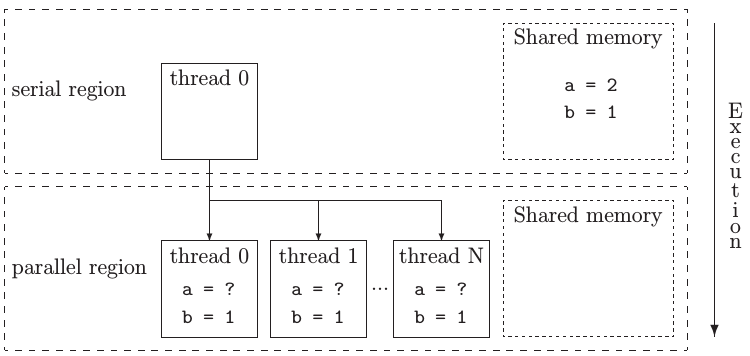
\includegraphics[width=0.80\textwidth]{figuras/reg-paralelaValPriv.png} \\
  \caption{Representaci\'on gr\'afica de las cl\'ausulas PRIVATE y FIRSTPRIVATE.} %
  \label{figRegparVarPriv}
\end{figure}

Al incluir la variable en una cl\'ausula FIRSTPRIVATE al inicio del alcance de una directiva toma autom\'aticamente el estatus de PRIVATE en dicho alcance y no es necesario incluirla en una cl\'ausula PRIVATE expl\'icitamente.
Al igual que con las variables PRIVATE debe tenerse en cuenta el costo de la operaci\'on desde el punto de vista computacional, al realizarse una copia de la variable y transferir la informaci\'on almacenada a la nueva variable.

\subsection{Otras Construcciones y Cl\'ausulas}
Existen m\'as construcciones de trabajo compartido, de sincronizaci\'on y de ambiente de datos, y m\'as cl\'ausulas en OpenMP, las cuales exceden el alcance de este trabajo de tesis y que pueden ser consultadas en el est\'andar OpenMP\citep{openmp} o en \citep{Her}.

\section{Proceso de optimizaci\'on}\label{sec:n6}
Dependiendo del prop\'osito de una aplicaci\'on, y de la forma como ser\'a utilizada, suelen considerarse tres principios de optimizaci\'on del desempe\~no\citep{Garg}
\begin{itemize}
\item Resolver el problema m\'as r\'apidamente
\item Resolver un problema m\'as grande en el mismo tiempo
\item Resolver el mismo problema en el mismo tiempo, pero utilizando una cantidad menor de recursos del sistema
\end{itemize}
En aplicaciones de HPC, obtener resultados m\'as r\'apidamente es crucial para los usuarios. Por ejemplo, para un ingeniero, representa una diferencia considerable poder repetir una simulaci\'on en el transcurso de una noche en lugar de esperar varios d\'ias para que la simulaci\'on termine. El tiempo ganado puede ser aprovechado para modificar el dise\~no, correr experimentos de mayor tama\~no, resolver problemas con conjuntos de datos m\'as grandes, u obtener resultados m\'as precisos. Por otro lado, cuando el tama\~no del problema y el tiempo de ejecuci\'on se mantengan constantes, una aplicaci\'on optimizada consumir\'a menos recursos para completar su ejecuci\'on\citep{Garg}.

El proceso de optimizaci\'on tiene algunas etapas fundamentales: ``desarrollo de la aplicaci\'on, optimizaci\'on serial, y optimizaci\'on paralela''.  La primera etapa abarca el dise\~no, programaci\'on y consideraciones de portabilidad de la aplicaci\'on, es decir, elecci\'on de algoritmos y estructuras de datos para resolver el problema. En el caso de este trabajo de tesis, esa etapa fue llevada a cabo por el autor de la aplicaci\'on en que basamos nuestro estudio. Las etapas de optimizaci\'on serial y optimizaci\'on paralela son las que ser\'an explicadas brevemente en esta subsecci\'on. En la Fig. \ref{figGySEtapas} perteneciente a \citep{Garg}, podemos observar las etapas del proceso de optimizaci\'on.

Una decisi\'on importante para el proceso de optimizaci\'on es contemplar en qu\'e plataforma o conjunto de ellas se implementar\'a la aplicaci\'on. Esta decisi\'on incluye seleccionar sistema operativo y arquitectura de ejecuci\'on. La optimizaci\'on ser\'a m\'as focalizada mientras m\'as puntuales sean las decisiones tomadas, limitando el rango de plataformas en las cuales el programa puede ejecutarse\citep{Garg}. Una vez que el programa produzca resultados correctos, estar\'a listo para ser optimizado. Se seleccionar\'an un conjunto de casos de test para validar que el programa contin\'ue arrojando resultados correctos y se los utilizar\'a repetidamente en el transcurso de la optimizaci\'on.

\begin{figure}[htb]%[htp]
  \centering
  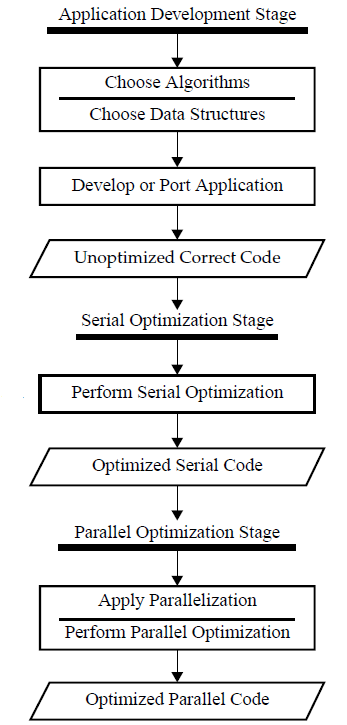
\includegraphics[width=0.40\textwidth]{figuras/g-and-s-etapas1.png} \\
  \caption{Etapas de Optimizaci\'on y Desarrollo de una Aplicaci\'on.} %
   \label{figGySEtapas}
\end{figure}

Tambi\'en se debe seleccionar un conjunto de casos para llevar a cabo pruebas de tiempo. Puede ser necesario que este conjunto sea diferente a los utilizados para validar el programa. Los casos de test para el cronometraje de tiempo podr\'ian ser varios ``benchmarks'' que representen adecuadamente el uso del programa. Se utilizar\'an estos benchmarks para medir el nivel de desempe\~no b\'asico o ``l\'inea de base'', de manera de disponer de datos fiables para utilizar m\'as tarde en las comparaciones de c\'odigo optimizado y c\'odigo original. De esta manera, se puede medir el efecto de la optimizaci\'on.

\subsection{Optimizaci\'on Serial}
La Optimizaci\'on Serial es un proceso iterativo que involucra medir repetidamente un programa seguido por la optimizaci\'on de sus partes cr\'iticas de rendimiento. La Fig. \ref{figGySSerial} tomada de \citep{Garg} resume las tareas de optimizaci\'on y da un diagrama de flujo simplificado para el proceso de optimizaci\'on serial.

\begin{figure}[h!]%[htp]
  \centering
  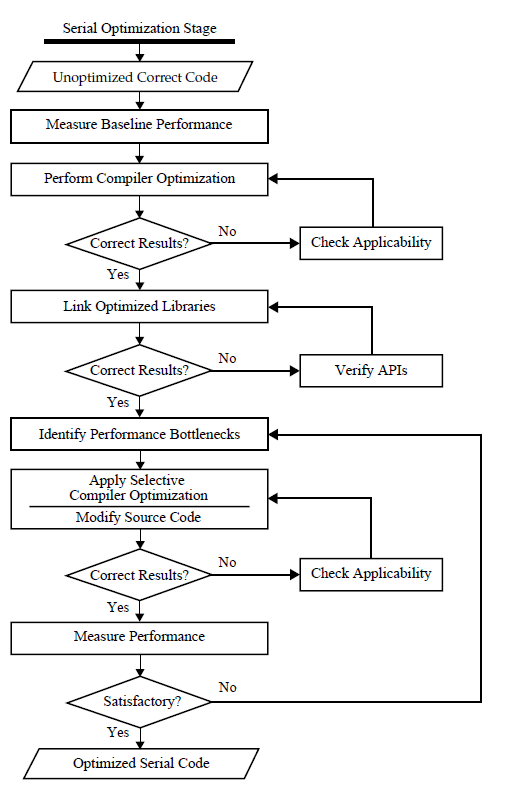
\includegraphics[width=0.60\textwidth]{figuras/g-and-s-serial1.png} \\
  \caption{Proceso de Optimizaci\'on Serial.} %
  \label{figGySSerial}
\end{figure}

Una vez que las mediciones de rendimiento de la l\'inea de base se han obtenido, el esfuerzo de optimizaci\'on debe iniciarse mediante la compilaci\'on de todo el programa con opciones seguras. Siguiente, linkear librer\'ias optimizadas. (Este linkeo es una manera sencilla de llevar implementaciones altamente optimizadas de operaciones estandar en un programa)
Luego de esto se debe verificar que los resultados preservan la correctitud del programa. Este paso incluye verificar que el programa realiza llamadas a las Interfaces de Programaci\'on de Aplicaci\'on (APIs sus siglas en Ingles) adecuadas en las librer\'ias optimizadas. Adem\'as, es recomendable que sea medido el desempe\~no del programa para verificar que ha mejorado.

El siguiente paso es identificar partes de desempe\~no cr\'iticas en el c\'odigo. El perfilado (profiling en Ingles) del c\'odigo fuente puede ser usado para determinar cuales partes del c\'odigo son las que toman m\'as tiempo para ejecutarse. Las partes identificadas son excelentes objetivos para enfocar el esfuerzo de optimizaci\'on, y las mejoras resultantes de desempe\~no pueden ser significativas. Otra t\'ecnica muy \'util para identificar estas partes de c\'odigo cr\'iticas es el monitoreo de la actividad del sistema y el uso de los recursos del sistema\citep{Garg}. 

\subsubsection{Metodolog\'ia de medici\'on}
Al trabajar en optimizar la performance de una aplicaci\'on, es esencial usar varias herramientas y t\'ecnicas que sugieran que partes del programa necesitan ser optimizadas, comparar el desempe\~no antes y luego de la optimizaci\'on y mostrar que tan eficiente los recursos del sistema han sido utilizados por el c\'odigo optimizado\citep{Garg}.

El primer paso en el proceso de afinaci\'on de la aplicaci\'on es cuantificar su desempe\~no. Este paso es alcanzado usualmente estableciendo un desempe\~no base y fijando expectativas apropiadas de cuanta mejora en el desempe\~no es razonable alcanzar.
Para programas cientificos, la m\'etricas de mayor inter\'es son usualmente el tiempo reloj (tiempo de respuesta) de un solo trabajo y aquellos que relacionan el desempe\~no de la aplicaci\'on a picos te\'oricos de desempe\~no de la CPU\citep{Garg}.
A traves de benchmarks es que podemos realizar an\'alisis de la performance de la aplicaci\'on. Una gu\'ia importante a seguir es que las mediciones deben ser reproducibles dentro de un rango de tolerancia esperado. Con esto en mente se definen las siguientes reglas generales:
\begin{itemize}
\item Seleccionar cuidadosamente los conjuntos de datos a utilizar. Deben representar adecuadamente el uso de la aplicaci\'on.
\item Al igual que en las mediciones en otros campos de la ingenier\'ia, la incertidumbre tambi\'en se aplica a las mediciones de desempe\~no de programas de computadora. El simple hecho de tratar de medir un programa se entromete en su ejecuci\'on y posiblemente lo afecta de manera incierta.
\item Siempre que sea posible, ejecutar los benchmarks desde un sistema de archivos tipo tmpfs (/tmp) o alg\'un sistema de archivos montado localmente. Ejecutar una aplicaci\'on desde un sistema de archivos montado por red introduce efectos de red irreproducibles en el tiempo de ejecuci\'on.
\item Actividades de paginado y swapeo deben ser monitoreadas mientras se ejecuta el benchmark, ya que estas pueden desvirtuar completamente la medici\'on.
\item Las mediciones de ``respuesta del programa'' deben ser desempe\~nadas en una manera dedicada, sin otros programas o aplicaciones ejecutandose.
\item Las caracteristicas del sistema deben ser registradas y guardadas.
\end{itemize}

\subsubsection{Herramientas de medici\'on}
Antes de analizar el desempe\~no de la aplicaci\'on, uno debe identificar los parametros que deben ser medidos y elegir herramientas acordes a las mediciones.
Las herramientas de medici\'on de desempe\~no pueden ser divididas en tres grupos\citep{Garg} basados en su funci\'on:
\begin{itemize}
\item Herramientas de temporizador, que miden el tiempo utilizado por un programa de usuario o sus partes. Pueden ser herramientas de l\'inea de comando o funciones dentro del programa.
\item Herramientas de perfilado, que utilizan resultados de tiempo para identificar las partes de mayor utilizaci\'on de una aplicaci\'on.
\item Herramientas de monitoreo, que miden la utilizaci\'on de varios recursos del sistema para identificar ``cuellos de botella'' que ocurren durante la ejecuci\'on.
\end{itemize}
Existen otras formas de categorizar estas herramientas, como puede ser basados en los requerimientos para su uso (herramientas que operan con binarios optimizados, o que requieren insertarse en el c\'odigo fuente, etc), o incluso dividirlas en dos grupos:
\begin{itemize}
\item Herramientas de medici\'on de desempe\~no serial
\item Herramientas de medici\'on de desempe\~no paralelo.
\end{itemize}

\subsubsection{Herramientas de medici\'on de tiempo}
El paso fundamental para evaluar comparativamente y poner a punto el desempe\~no de un programa es medir con precisi\'on la cantidad de tiempo utilizado ejecutando el c\'odigo. Generalmente uno est\'a interesado en el tiempo total utilizado para correr un programa, as\'i como en el tiempo utilizado en porciones del programa.
Para medir el programa completo es necesario usar herramientas que midan con precisi\'on el tiempo transcurrido desde el comienzo de la ejecuci\'on del programa. En GNU/Linux utilizamos la herramienta ``time'' para dicho prop\'osito. La forma de utilizar time es ejecutarlo desde una terminal de GNU/Linux pasando como par\'ametro el comando que debe medir tal cual como el comando es ejecutado normalmente. Por ejemplo:
\begin{lstlisting}[style=For, numbers=none]
	$ time  find / -name ``syslog''
\end{lstlisting}
El comando siendo medido realiza su ejecuci\'on normalmente. Al finalizar su ejecuci\'on, el comando time muestra por salida est\'andar tres valores (Fig. \ref{figTime}):
\begin{itemize}
\item ``real'': el tiempo real transcurrido entre el inicio y la finalizaci\'on de la ejecuci\'on.
\item ``user'': el tiempo de usuario del procesador.
\item ``sys'': el tiempo de sistema del procesador.
\end{itemize}

\begin{figure}[htbp]
  \begin{lstlisting}[style=consola, numbers=none]
  h4ndr3s@gondolin:~$ time find . -name "invisidos*"
  ./t3sis/tesis/source/invisidos2fin.for
  ./t3sis/tesis/source/invisidos2fin_OMP_def.for
  ./t3sis/tesis/source/invisidos2fin_OMP-origfuncionando.for
  ./t3sis/tesis/source/invisidos2fin_OMP_80.for

  real    0m0.089s
  user    0m0.060s
  sys     0m0.024s
  \end{lstlisting}
  \caption{Ejemplo de ejecuci\'on del comando \emph{time}.} %
  \label{figTime}
\end{figure}

\subsubsection{Herramientas de perfilado de programa}
El perfilado muestra cuales funciones son las m\'as costosas en las ejecuciones de una aplicaci\'on. Es necesario utilizar para la medici\'on casos de test representativos y multiples, de manera de obtener resultados significativos.
En GNU/Linux se cuenta con la herramienta ``gprof'' para realizar perfilado de aplicaciones. Para utilizarla un programa debe estar compilada con la opci\'on ``-pg''. Luego se ejecuta el programa una vez y genera un archivo llamado gmon.out en el directorio de ejecuci\'on el cual es utilizado por el comando gprof para generar el reporte de perfilado para esa ejecuci\'on. La sintaxis de gprof es:
\begin{lstlisting}[style=For, numbers=none]
	$ gprof  <programa_ejecutable>  [<ruta_a_gmon.out>]
\end{lstlisting}
Si no se le pasa la ruta a gmon.out, por defecto utiliza el directorio desde donde es invocado gprof. Un ejemplo de este proceso puede verse a continuaci\'on: 

\begin{lstlisting}[style=For, numbers=none]
    $ gfortran -pg foo.for -o foo
    $ foo
    $ gprof foo
\end{lstlisting}
La salida de gprof es por salida est\'andar y bastante extensa, por lo cual es aconsejable redirigirla a un archivo. Consta de tres partes: la primera parte lista las funciones ordenadas de acuerdo al tiempo que consumen, junto con sus descendientes (tiempo inclusivo). La segunda parte lista el tiempo exclusivo para las funciones (tiempo empleado ejecutando la funci\'on) junto con los porcentajes de tiempo total de ejecuci\'on y n\'umero de llamadas. La \'ultima parte da un \'indice de todas las llamadas realizadas en la ejecuci\'on.

\subsection{Optimizaci\'on Paralela}
Luego de que la aplicaci\'on est\'a optimizada para procesamiento secuencial, su tiempo de ejecuci\'on puede ser  reducido a\'un m\'as permitiendo que se ejecute en varios procesadores. Las t\'ecnicas m\'as usadas comunmente para paralelizaci\'on son el uso expl\'icito de hilos, el uso de directivas al compilador y el pasaje de mensajes\citep{Garg}. En la Fig. \ref{figGySParalel} de \citep{Garg} se v\'e ilustrado el proceso de optimizaci\'on paralela.

\begin{figure}[h!]%[htp]
  \centering
  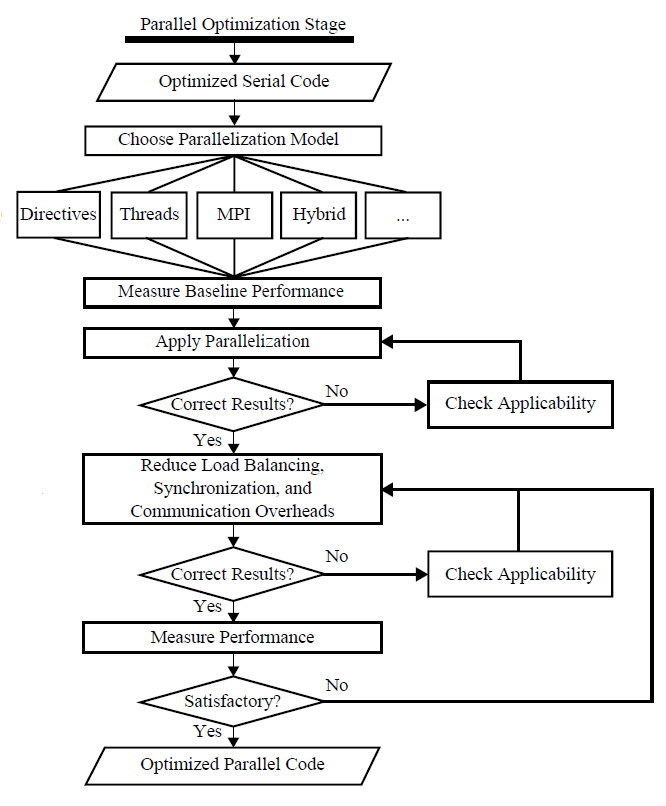
\includegraphics[width=0.65\textwidth]{figuras/g-and-s-paralel1.png} \\
  \caption{Proceso de Optimizaci\'on Paralela.} %
  \label{figGySParalel}
\end{figure}

El primer paso es elegir un modelo, identificar que partes del programa deben ser paralelizadas y determinar como dividir la carga de trabajo computacional entre los diferentes procesadores. Dividir la carga de trabajo computacional es crucial para el desempe\~no, ya que determina los gastos generales de comunicaci\'on, sincronizaci\'on y de desequilibrios de carga resultantes en un programa paralelizado. Generalmente, una divisi\'on de trabajo de ``nivel grueso'' es recomendada debido a que minimiza la comunicaci\'on entre las tareas paralelas, pero en algunos casos, un enfoque de este tipo lleva a balanceo de carga muy pobre; un nivel m\'as fino en el particionamiento de la carga de trabajo puede llevar a un mejor balanceo de carga y desempe\~no de la aplicaci\'on.

Luego de seleccionado un modelo de paralelizaci\'on e implementado, lo siguiente es optimizar su desempe\~no. Similar a la optimizaci\'on serial, este proceso es iterativo e involucra mediciones repetidas seguidas de aplicar una o m\'as t\'ecnicas de optimizaci\'on para mejorar el desempe\~no del programa. Las aplicaciones paralelas, sin importar el modelo utilizado, necesitan que exista comunicaci\'on entre los procesos o hilos concurrentes. Se debe tener cuidado de minimizar los gastos extras en comunicaci\'on y asegurar una sincronizaci\'on eficiente en la implementaci\'on; Minimizar el desequilibrio de cargas entre las tareas paralelas, ya que esto degrada la escalabilidad del programa. Tambi\'en se debe considerar temas como migraci\'on y programaci\'on de procesos, y coherencia de cache. Las librer\'ias del compilador pueden ser utilizadas para implementar versiones paralelas de funciones usadas comunmente, tanto en aplicaciones multihilo como multiproceso.

Los cuellos de botella de un programa paralelo pueden ser muy diferentes de los presentes en una versi\'on secuencial del mismo programa. Adem\'as de gastos extras espec\'ificos de la paralelizaci\'on, las porciones lineales (o secuenciales) de un programa paralelo pueden limitar severamente la ganancia de velocidad de la paralelizaci\'on. En tales situaciones , hay que prestar atenci\'on a esas porciones secuenciales para mejorar el desempe\~no total de la aplicaci\'on paralela. Por ejemplo, consideremos la soluci\'on directa de N ecuaciones lineales. El costo computacional escala en el orden de O(N\sptext{3}) en la etapa de descomposici\'on de la matriz y en el orden de O(N\sptext{2}) en la etapa de sustituci\'on adelante-atr\'as. En consecuencia, la etapa de sustituci\'on adelante-atr\'as apenas se nota en el programa secuencial, y el desarrollador paralelizando el programa justificadamente se enfoca en la etapa de descomposici\'on de la matriz. Posiblemente, como resultado del trabajo de paralelizaci\'on, la etapa de descomposici\'on de la matriz se vuelve m\'as eficiente que la etapa de sustituci\'on adelante-atr\'as. El desempe\~no total y velocidad del programa de resoluci\'on directa ahora est\'a limitado por el desempe\~no de la etapa de sustituci\'on adelante-atr\'as. Para mejorar a\'un m\'as el desempe\~no, la etapa de sustituci\'on adelante-atr\'as deber\'ia convertirse en el foco de optimizaci\'on y posiblemente un trabajo de paralelizaci\'on\citep{Garg}.

\section{Caso de Estudio: Modelizaci\'on del Flujo Inv\'iscido}\label{sec:n7}
El programa objeto de optimizaci\'on de esta tesis es de autor\'ia de Ricardo A. Prado, docente e investigador de la Universidad Nacional del Comahue, y fue utilizado para obtener resultados para su trabajo de tesis de doctorado\citep[Mayo 2007]{Prado} en el \'area de Ingenier\'ia presentado en la Universidad de Buenos Aires en 2007. Como se expone en dicho trabajo, la tesis ``analiza el comportamiento fluidodin\'amico de una turbom\'aquina particular: la turbina e\'olica''. La creaci\'on del programa se justifica en el mismo trabajo porque ``debido a la complejidad de las ecuaciones de gobierno en ambas zonas del campo fluidodin\'amico, como as\'i tambi\'en de la geometr\'ia de la turbina y de sus condiciones de operaci\'on, se requiere de procesos de resoluci\'on num\'erica adecuados, los cuales se incorporaron en los c\'odigos computacionales que se desarrollaron a tal efecto''.

El modelo matem\'atico que implementa el programa es la ``Ley de Biot-Savart'', que indica el campo magn\'etico creado por corrientes el\'ectricas estacionarias. Es una de las leyes fundamentales de la magnetoest\'atica. En particular, en el trabajo de Prado se aplica a una modelizaci\'on del flujo inv\'iscido (de viscosidad despreciable, casi nula) alrededor de la pala de la turbina. El modelo num\'erico se formula a trav\'es del m\'etodo de los paneles. El objetivo de la aplicaci\'on de la Ley de Biot-Savart en el trabajo es el c\'alculo de las velocidades de flujo inducidas en un punto para cada panel de la pala. 

El programa realiza el c\'alculo de una integraci\'on por el m\'etodo de Simpson. La regla o m\'etodo de Simpson es un m\'etodo de integraci\'on num\'erica que se utiliza para obtener la aproximaci\'on de una integral en un intervalo definido, al dividir ese intervalo en subintervalos y aproximar cada subintervalo con un polinomio de segundo grado. 